\documentclass[twoside]{book}

% Packages required by doxygen
\usepackage{fixltx2e}
\usepackage{calc}
\usepackage{doxygen}
\usepackage[export]{adjustbox} % also loads graphicx
\usepackage{graphicx}
\usepackage[utf8]{inputenc}
\usepackage{makeidx}
\usepackage{multicol}
\usepackage{multirow}
\PassOptionsToPackage{warn}{textcomp}
\usepackage{textcomp}
\usepackage[nointegrals]{wasysym}
\usepackage[table]{xcolor}

% Font selection
\usepackage[T1]{fontenc}
\usepackage[scaled=.90]{helvet}
\usepackage{courier}
\usepackage{amssymb}
\usepackage{sectsty}
\renewcommand{\familydefault}{\sfdefault}
\allsectionsfont{%
  \fontseries{bc}\selectfont%
  \color{darkgray}%
}
\renewcommand{\DoxyLabelFont}{%
  \fontseries{bc}\selectfont%
  \color{darkgray}%
}
\newcommand{\+}{\discretionary{\mbox{\scriptsize$\hookleftarrow$}}{}{}}

% Page & text layout
\usepackage{geometry}
\geometry{%
  a4paper,%
  top=2.5cm,%
  bottom=2.5cm,%
  left=2.5cm,%
  right=2.5cm%
}
\tolerance=750
\hfuzz=15pt
\hbadness=750
\setlength{\emergencystretch}{15pt}
\setlength{\parindent}{0cm}
\setlength{\parskip}{0.2cm}
\makeatletter
\renewcommand{\paragraph}{%
  \@startsection{paragraph}{4}{0ex}{-1.0ex}{1.0ex}{%
    \normalfont\normalsize\bfseries\SS@parafont%
  }%
}
\renewcommand{\subparagraph}{%
  \@startsection{subparagraph}{5}{0ex}{-1.0ex}{1.0ex}{%
    \normalfont\normalsize\bfseries\SS@subparafont%
  }%
}
\makeatother

% Headers & footers
\usepackage{fancyhdr}
\pagestyle{fancyplain}
\fancyhead[LE]{\fancyplain{}{\bfseries\thepage}}
\fancyhead[CE]{\fancyplain{}{}}
\fancyhead[RE]{\fancyplain{}{\bfseries\leftmark}}
\fancyhead[LO]{\fancyplain{}{\bfseries\rightmark}}
\fancyhead[CO]{\fancyplain{}{}}
\fancyhead[RO]{\fancyplain{}{\bfseries\thepage}}
\fancyfoot[LE]{\fancyplain{}{}}
\fancyfoot[CE]{\fancyplain{}{}}
\fancyfoot[RE]{\fancyplain{}{\bfseries\scriptsize Generated on Wed Jan 27 2016 20\+:55\+:05 for Rhino by Doxygen }}
\fancyfoot[LO]{\fancyplain{}{\bfseries\scriptsize Generated on Wed Jan 27 2016 20\+:55\+:05 for Rhino by Doxygen }}
\fancyfoot[CO]{\fancyplain{}{}}
\fancyfoot[RO]{\fancyplain{}{}}
\renewcommand{\footrulewidth}{0.4pt}
\renewcommand{\chaptermark}[1]{%
  \markboth{#1}{}%
}
\renewcommand{\sectionmark}[1]{%
  \markright{\thesection\ #1}%
}

% Indices & bibliography
\usepackage{natbib}
\usepackage[titles]{tocloft}
\setcounter{tocdepth}{3}
\setcounter{secnumdepth}{5}
\makeindex

% Hyperlinks (required, but should be loaded last)
\usepackage{ifpdf}
\ifpdf
  \usepackage[pdftex,pagebackref=true]{hyperref}
\else
  \usepackage[ps2pdf,pagebackref=true]{hyperref}
\fi
\hypersetup{%
  colorlinks=true,%
  linkcolor=blue,%
  citecolor=blue,%
  unicode%
}

% Custom commands
\newcommand{\clearemptydoublepage}{%
  \newpage{\pagestyle{empty}\cleardoublepage}%
}


%===== C O N T E N T S =====

\begin{document}

% Titlepage & ToC
\hypersetup{pageanchor=false,
             bookmarks=true,
             bookmarksnumbered=true,
             pdfencoding=unicode
            }
\pagenumbering{roman}
\begin{titlepage}
\vspace*{7cm}
\begin{center}%
{\Large Rhino }\\
\vspace*{1cm}
{\large Generated by Doxygen 1.8.9.1}\\
\vspace*{0.5cm}
{\small Wed Jan 27 2016 20:55:05}\\
\end{center}
\end{titlepage}
\clearemptydoublepage
\tableofcontents
\clearemptydoublepage
\pagenumbering{arabic}
\hypersetup{pageanchor=true}

%--- Begin generated contents ---
\chapter{Data Structure Index}
\section{Data Structures}
Here are the data structures with brief descriptions\+:\begin{DoxyCompactList}
\item\contentsline{section}{\hyperlink{struct__rqhd__args}{\+\_\+rqhd\+\_\+args} \\*Request handler, request arguments }{\pageref{struct__rqhd__args}}{}
\item\contentsline{section}{\hyperlink{struct__rqhd__header}{\+\_\+rqhd\+\_\+header} \\*Request handler, respons header }{\pageref{struct__rqhd__header}}{}
\item\contentsline{section}{\hyperlink{struct__rqhd__req}{\+\_\+rqhd\+\_\+req} \\*Request handler, request data }{\pageref{struct__rqhd__req}}{}
\item\contentsline{section}{\hyperlink{struct__rqhd__req__head}{\+\_\+rqhd\+\_\+req\+\_\+head} \\*Request handler, request header }{\pageref{struct__rqhd__req__head}}{}
\item\contentsline{section}{\hyperlink{structconfiguration}{configuration} \\*Config structures }{\pageref{structconfiguration}}{}
\item\contentsline{section}{\hyperlink{structyy__buffer__state}{yy\+\_\+buffer\+\_\+state} }{\pageref{structyy__buffer__state}}{}
\item\contentsline{section}{\hyperlink{structyy__trans__info}{yy\+\_\+trans\+\_\+info} }{\pageref{structyy__trans__info}}{}
\end{DoxyCompactList}

\chapter{Data Structure Documentation}
\hypertarget{struct__rqhd__args}{}\section{\+\_\+rqhd\+\_\+args Struct Reference}
\label{struct__rqhd__args}\index{\+\_\+rqhd\+\_\+args@{\+\_\+rqhd\+\_\+args}}


Request handler, request arguments.  




{\ttfamily \#include $<$structures.\+h$>$}



Collaboration diagram for \+\_\+rqhd\+\_\+args\+:
\nopagebreak
\begin{figure}[H]
\begin{center}
\leavevmode
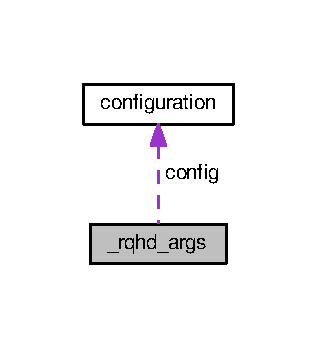
\includegraphics[width=152pt]{struct__rqhd__args__coll__graph}
\end{center}
\end{figure}
\subsection*{Data Fields}
\begin{DoxyCompactItemize}
\item 
\hypertarget{struct__rqhd__args_a8a362ad4d44ca6a1cf7632552ad83906}{}int {\bfseries sd}\label{struct__rqhd__args_a8a362ad4d44ca6a1cf7632552ad83906}

\item 
\hypertarget{struct__rqhd__args_a22ab4fcf3d0f952989272fc389bb0f10}{}struct sockaddr\+\_\+in {\bfseries pin}\label{struct__rqhd__args_a22ab4fcf3d0f952989272fc389bb0f10}

\item 
\hypertarget{struct__rqhd__args_a0e9770e8c53d9c99ee6943f58ff11216}{}\hyperlink{structconfiguration}{configuration} $\ast$ {\bfseries config}\label{struct__rqhd__args_a0e9770e8c53d9c99ee6943f58ff11216}

\end{DoxyCompactItemize}


\subsection{Detailed Description}
Request handler, request arguments. 

The documentation for this struct was generated from the following file\+:\begin{DoxyCompactItemize}
\item 
/home/jim/\+Documents/\+Git\+Hub/\+Rhino/webserver/include/structures.\+h\end{DoxyCompactItemize}

\hypertarget{struct__rqhd__header}{}\section{\+\_\+rqhd\+\_\+header Struct Reference}
\label{struct__rqhd__header}\index{\+\_\+rqhd\+\_\+header@{\+\_\+rqhd\+\_\+header}}


Request handler, respons header.  




{\ttfamily \#include $<$structures.\+h$>$}

\subsection*{Data Fields}
\begin{DoxyCompactItemize}
\item 
\hypertarget{struct__rqhd__header_a9b27a9d853f6b86c89e14dcc97a02b84}{}char {\bfseries protocol} \mbox{[}B\+U\+F\+\_\+\+V\+A\+L\mbox{]}\label{struct__rqhd__header_a9b27a9d853f6b86c89e14dcc97a02b84}

\item 
\hypertarget{struct__rqhd__header_a2350182ce9e30aa1b907de0779cff24a}{}char {\bfseries status} \mbox{[}B\+U\+F\+\_\+\+V\+A\+L\mbox{]}\label{struct__rqhd__header_a2350182ce9e30aa1b907de0779cff24a}

\item 
\hypertarget{struct__rqhd__header_a23bc223de49974b82ece89cd8a80f642}{}char {\bfseries server} \mbox{[}B\+U\+F\+\_\+\+V\+A\+L\mbox{]}\label{struct__rqhd__header_a23bc223de49974b82ece89cd8a80f642}

\item 
\hypertarget{struct__rqhd__header_ad1ea6613159c6c20dfd7427041428def}{}char {\bfseries type} \mbox{[}B\+U\+F\+\_\+\+V\+A\+L\mbox{]}\label{struct__rqhd__header_ad1ea6613159c6c20dfd7427041428def}

\item 
\hypertarget{struct__rqhd__header_aa624b6831909b55f315899b315f256e8}{}char {\bfseries cache} \mbox{[}B\+U\+F\+\_\+\+V\+A\+L\mbox{]}\label{struct__rqhd__header_aa624b6831909b55f315899b315f256e8}

\item 
\hypertarget{struct__rqhd__header_a66208b4829ec43bb54a650df71b0b642}{}char {\bfseries modified} \mbox{[}B\+U\+F\+\_\+\+V\+A\+L\mbox{]}\label{struct__rqhd__header_a66208b4829ec43bb54a650df71b0b642}

\item 
\hypertarget{struct__rqhd__header_a4e83bf48a4ef0a06ee55867bfd1650a5}{}int {\bfseries size}\label{struct__rqhd__header_a4e83bf48a4ef0a06ee55867bfd1650a5}

\end{DoxyCompactItemize}


\subsection{Detailed Description}
Request handler, respons header. 

The documentation for this struct was generated from the following file\+:\begin{DoxyCompactItemize}
\item 
/home/jim/\+Documents/\+Git\+Hub/\+Rhino/webserver/include/structures.\+h\end{DoxyCompactItemize}

\hypertarget{struct__rqhd__req}{}\section{\+\_\+rqhd\+\_\+req Struct Reference}
\label{struct__rqhd__req}\index{\+\_\+rqhd\+\_\+req@{\+\_\+rqhd\+\_\+req}}


Request handler, request data.  




{\ttfamily \#include $<$structures.\+h$>$}



Collaboration diagram for \+\_\+rqhd\+\_\+req\+:
\nopagebreak
\begin{figure}[H]
\begin{center}
\leavevmode
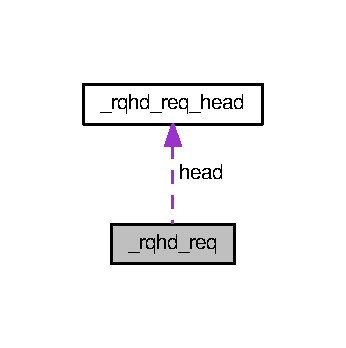
\includegraphics[width=166pt]{struct__rqhd__req__coll__graph}
\end{center}
\end{figure}
\subsection*{Data Fields}
\begin{DoxyCompactItemize}
\item 
\hypertarget{struct__rqhd__req_a185edae62d9cb48cbe295194f1fb5983}{}char {\bfseries method} \mbox{[}B\+U\+F\+\_\+\+V\+A\+L\mbox{]}\label{struct__rqhd__req_a185edae62d9cb48cbe295194f1fb5983}

\item 
\hypertarget{struct__rqhd__req_aac2e28a7a9619316e495bdd26784c8b4}{}char {\bfseries uri} \mbox{[}B\+U\+F\+\_\+\+V\+A\+L\mbox{]}\label{struct__rqhd__req_aac2e28a7a9619316e495bdd26784c8b4}

\item 
\hypertarget{struct__rqhd__req_a1773c26caba4f8950d9c0fa079f0f63f}{}char {\bfseries path} \mbox{[}B\+U\+F\+\_\+\+V\+A\+L\mbox{]}\label{struct__rqhd__req_a1773c26caba4f8950d9c0fa079f0f63f}

\item 
\hypertarget{struct__rqhd__req_a907b7f03e190c20d7bbfcec7c0422d45}{}char {\bfseries protocol} \mbox{[}B\+U\+F\+\_\+\+V\+A\+L\mbox{]}\label{struct__rqhd__req_a907b7f03e190c20d7bbfcec7c0422d45}

\item 
\hypertarget{struct__rqhd__req_a251a5ca4b38705026711bccff3827afe}{}\hyperlink{struct__rqhd__req__head}{\+\_\+rqhd\+\_\+req\+\_\+head} {\bfseries head}\label{struct__rqhd__req_a251a5ca4b38705026711bccff3827afe}

\item 
\hypertarget{struct__rqhd__req_a01245ed1c86c65c1a5de9f942a132f5d}{}bool {\bfseries error}\label{struct__rqhd__req_a01245ed1c86c65c1a5de9f942a132f5d}

\end{DoxyCompactItemize}


\subsection{Detailed Description}
Request handler, request data. 

The documentation for this struct was generated from the following file\+:\begin{DoxyCompactItemize}
\item 
/home/jim/\+Documents/\+Git\+Hub/\+Rhino/webserver/include/structures.\+h\end{DoxyCompactItemize}

\hypertarget{struct__rqhd__req__head}{}\section{\+\_\+rqhd\+\_\+req\+\_\+head Struct Reference}
\label{struct__rqhd__req__head}\index{\+\_\+rqhd\+\_\+req\+\_\+head@{\+\_\+rqhd\+\_\+req\+\_\+head}}


Request handler, request header.  




{\ttfamily \#include $<$structures.\+h$>$}

\subsection*{Data Fields}
\begin{DoxyCompactItemize}
\item 
\hypertarget{struct__rqhd__req__head_a038f132d35efc004445dd675509a6646}{}char {\bfseries host} \mbox{[}B\+U\+F\+\_\+\+V\+A\+L\mbox{]}\label{struct__rqhd__req__head_a038f132d35efc004445dd675509a6646}

\item 
\hypertarget{struct__rqhd__req__head_af61412bb4bc6ab6676c6b455f755ae4f}{}char {\bfseries user\+Agent} \mbox{[}B\+U\+F\+\_\+\+V\+A\+L\mbox{]}\label{struct__rqhd__req__head_af61412bb4bc6ab6676c6b455f755ae4f}

\item 
\hypertarget{struct__rqhd__req__head_ae9a856190aaa572d51743ecfe9804624}{}char {\bfseries accept} \mbox{[}B\+U\+F\+\_\+\+V\+A\+L\mbox{]}\label{struct__rqhd__req__head_ae9a856190aaa572d51743ecfe9804624}

\item 
\hypertarget{struct__rqhd__req__head_a023b09ff3a60ba158a59a46caa38a12c}{}char {\bfseries referer} \mbox{[}B\+U\+F\+\_\+\+V\+A\+L\mbox{]}\label{struct__rqhd__req__head_a023b09ff3a60ba158a59a46caa38a12c}

\end{DoxyCompactItemize}


\subsection{Detailed Description}
Request handler, request header. 

The documentation for this struct was generated from the following file\+:\begin{DoxyCompactItemize}
\item 
/home/jim/\+Documents/\+Git\+Hub/\+Rhino/webserver/include/structures.\+h\end{DoxyCompactItemize}

\hypertarget{structconfiguration}{}\section{configuration Struct Reference}
\label{structconfiguration}\index{configuration@{configuration}}


Config structures.  




{\ttfamily \#include $<$structures.\+h$>$}

\subsection*{Data Fields}
\begin{DoxyCompactItemize}
\item 
\hypertarget{structconfiguration_aed0c9b94a011cb078df1af99d48e7aab}{}char {\bfseries servername} \mbox{[}B\+U\+F\+\_\+\+C\+F\+G\mbox{]}\label{structconfiguration_aed0c9b94a011cb078df1af99d48e7aab}

\item 
\hypertarget{structconfiguration_ad2fe27c15863d4fd985c3b5a7359cbea}{}char {\bfseries root\+Dir} \mbox{[}B\+U\+F\+\_\+\+C\+F\+G\mbox{]}\label{structconfiguration_ad2fe27c15863d4fd985c3b5a7359cbea}

\item 
\hypertarget{structconfiguration_ab336961b40adfa019461b001394cbf9a}{}char {\bfseries basedir} \mbox{[}B\+U\+F\+\_\+\+C\+F\+G\mbox{]}\label{structconfiguration_ab336961b40adfa019461b001394cbf9a}

\item 
\hypertarget{structconfiguration_ac01dc1f952cba461c7137e1bfb1bb9f7}{}char {\bfseries errpg} \mbox{[}B\+U\+F\+\_\+\+V\+A\+L\mbox{]}\label{structconfiguration_ac01dc1f952cba461c7137e1bfb1bb9f7}

\item 
\hypertarget{structconfiguration_a409fd0fd4c8759d40ced464cefa2aff4}{}char {\bfseries acc\+Log\+Path} \mbox{[}B\+U\+F\+\_\+\+C\+F\+G\mbox{]}\label{structconfiguration_a409fd0fd4c8759d40ced464cefa2aff4}

\item 
\hypertarget{structconfiguration_a3e8dfae545709fcf1dc87d4de01d2593}{}char {\bfseries srv\+Log\+Path} \mbox{[}B\+U\+F\+\_\+\+C\+F\+G\mbox{]}\label{structconfiguration_a3e8dfae545709fcf1dc87d4de01d2593}

\item 
\hypertarget{structconfiguration_aca60e65b2ec0893583b42607fb319b27}{}char {\bfseries config\+Path} \mbox{[}B\+U\+F\+\_\+\+C\+F\+G\mbox{]}\label{structconfiguration_aca60e65b2ec0893583b42607fb319b27}

\item 
\hypertarget{structconfiguration_ae245a0b0809a1d03125b14d6250e08ae}{}char {\bfseries fifo\+Path} \mbox{[}B\+U\+F\+\_\+\+C\+F\+G\mbox{]}\label{structconfiguration_ae245a0b0809a1d03125b14d6250e08ae}

\item 
\hypertarget{structconfiguration_aec617799bec821de03c3ba39120d53a4}{}int {\bfseries listen\+Port}\label{structconfiguration_aec617799bec821de03c3ba39120d53a4}

\item 
\hypertarget{structconfiguration_a393c7b28ae51b4d4388b7f815467cc68}{}int {\bfseries backlog}\label{structconfiguration_a393c7b28ae51b4d4388b7f815467cc68}

\item 
\hypertarget{structconfiguration_a0b6a3a095413154418f46056d13dad70}{}bool {\bfseries syslog}\label{structconfiguration_a0b6a3a095413154418f46056d13dad70}

\end{DoxyCompactItemize}


\subsection{Detailed Description}
Config structures. 

The documentation for this struct was generated from the following file\+:\begin{DoxyCompactItemize}
\item 
/home/jim/\+Documents/\+Git\+Hub/\+Rhino/webserver/include/structures.\+h\end{DoxyCompactItemize}

\hypertarget{structyy__buffer__state}{}\section{yy\+\_\+buffer\+\_\+state Struct Reference}
\label{structyy__buffer__state}\index{yy\+\_\+buffer\+\_\+state@{yy\+\_\+buffer\+\_\+state}}
\subsection*{Data Fields}
\begin{DoxyCompactItemize}
\item 
\hypertarget{structyy__buffer__state_a4360acfb226a1fc240ab2be17dd6beda}{}F\+I\+L\+E $\ast$ {\bfseries yy\+\_\+input\+\_\+file}\label{structyy__buffer__state_a4360acfb226a1fc240ab2be17dd6beda}

\item 
\hypertarget{structyy__buffer__state_a0d25458e69eb22207fc633a1255d099d}{}char $\ast$ {\bfseries yy\+\_\+ch\+\_\+buf}\label{structyy__buffer__state_a0d25458e69eb22207fc633a1255d099d}

\item 
\hypertarget{structyy__buffer__state_a8435c3f786bbb55d21d0174e4cfc22a0}{}char $\ast$ {\bfseries yy\+\_\+buf\+\_\+pos}\label{structyy__buffer__state_a8435c3f786bbb55d21d0174e4cfc22a0}

\item 
\hypertarget{structyy__buffer__state_a48302f5f3477a9c78bbddf56d356ef54}{}yy\+\_\+size\+\_\+t {\bfseries yy\+\_\+buf\+\_\+size}\label{structyy__buffer__state_a48302f5f3477a9c78bbddf56d356ef54}

\item 
\hypertarget{structyy__buffer__state_afcc44872643f513e79b43c2b1f334a67}{}yy\+\_\+size\+\_\+t {\bfseries yy\+\_\+n\+\_\+chars}\label{structyy__buffer__state_afcc44872643f513e79b43c2b1f334a67}

\item 
\hypertarget{structyy__buffer__state_a80ce2431c70dc4f89ced487f18449465}{}int {\bfseries yy\+\_\+is\+\_\+our\+\_\+buffer}\label{structyy__buffer__state_a80ce2431c70dc4f89ced487f18449465}

\item 
\hypertarget{structyy__buffer__state_abf5c70eea75581b58c0ee7bd31b14490}{}int {\bfseries yy\+\_\+is\+\_\+interactive}\label{structyy__buffer__state_abf5c70eea75581b58c0ee7bd31b14490}

\item 
\hypertarget{structyy__buffer__state_a9d60c60af6e1a6f69de16871fd64f85f}{}int {\bfseries yy\+\_\+at\+\_\+bol}\label{structyy__buffer__state_a9d60c60af6e1a6f69de16871fd64f85f}

\item 
int \hyperlink{structyy__buffer__state_a818e94bc9c766e683c60df1e9fd01199}{yy\+\_\+bs\+\_\+lineno}
\item 
int \hyperlink{structyy__buffer__state_a10c4fcd8be759e6bf11e6d3e8cdb0307}{yy\+\_\+bs\+\_\+column}
\item 
\hypertarget{structyy__buffer__state_a63d2afbb1d79a3fc63df9e12626f827d}{}int {\bfseries yy\+\_\+fill\+\_\+buffer}\label{structyy__buffer__state_a63d2afbb1d79a3fc63df9e12626f827d}

\item 
\hypertarget{structyy__buffer__state_a70fd925d37a2f0454fbd0def675d106c}{}int {\bfseries yy\+\_\+buffer\+\_\+status}\label{structyy__buffer__state_a70fd925d37a2f0454fbd0def675d106c}

\end{DoxyCompactItemize}


\subsection{Field Documentation}
\hypertarget{structyy__buffer__state_a10c4fcd8be759e6bf11e6d3e8cdb0307}{}\index{yy\+\_\+buffer\+\_\+state@{yy\+\_\+buffer\+\_\+state}!yy\+\_\+bs\+\_\+column@{yy\+\_\+bs\+\_\+column}}
\index{yy\+\_\+bs\+\_\+column@{yy\+\_\+bs\+\_\+column}!yy\+\_\+buffer\+\_\+state@{yy\+\_\+buffer\+\_\+state}}
\subsubsection[{yy\+\_\+bs\+\_\+column}]{\setlength{\rightskip}{0pt plus 5cm}int yy\+\_\+buffer\+\_\+state\+::yy\+\_\+bs\+\_\+column}\label{structyy__buffer__state_a10c4fcd8be759e6bf11e6d3e8cdb0307}
The column count. \hypertarget{structyy__buffer__state_a818e94bc9c766e683c60df1e9fd01199}{}\index{yy\+\_\+buffer\+\_\+state@{yy\+\_\+buffer\+\_\+state}!yy\+\_\+bs\+\_\+lineno@{yy\+\_\+bs\+\_\+lineno}}
\index{yy\+\_\+bs\+\_\+lineno@{yy\+\_\+bs\+\_\+lineno}!yy\+\_\+buffer\+\_\+state@{yy\+\_\+buffer\+\_\+state}}
\subsubsection[{yy\+\_\+bs\+\_\+lineno}]{\setlength{\rightskip}{0pt plus 5cm}int yy\+\_\+buffer\+\_\+state\+::yy\+\_\+bs\+\_\+lineno}\label{structyy__buffer__state_a818e94bc9c766e683c60df1e9fd01199}
The line count. 

The documentation for this struct was generated from the following files\+:\begin{DoxyCompactItemize}
\item 
/home/jim/\+Documents/\+Git\+Hub/\+Rhino/webserver/include/config\+Scanner.\+h\item 
/home/jim/\+Documents/\+Git\+Hub/\+Rhino/webserver/source/config\+Scanner.\+c\end{DoxyCompactItemize}

\hypertarget{structyy__trans__info}{}\section{yy\+\_\+trans\+\_\+info Struct Reference}
\label{structyy__trans__info}\index{yy\+\_\+trans\+\_\+info@{yy\+\_\+trans\+\_\+info}}
\subsection*{Data Fields}
\begin{DoxyCompactItemize}
\item 
\hypertarget{structyy__trans__info_a5c9f61e770deef50bd4e697310342fe9}{}flex\+\_\+int32\+\_\+t {\bfseries yy\+\_\+verify}\label{structyy__trans__info_a5c9f61e770deef50bd4e697310342fe9}

\item 
\hypertarget{structyy__trans__info_ae0715250c2bef261e596e77e0030f13e}{}flex\+\_\+int32\+\_\+t {\bfseries yy\+\_\+nxt}\label{structyy__trans__info_ae0715250c2bef261e596e77e0030f13e}

\end{DoxyCompactItemize}


The documentation for this struct was generated from the following file\+:\begin{DoxyCompactItemize}
\item 
/home/jim/\+Documents/\+Git\+Hub/\+Rhino/webserver/source/config\+Scanner.\+c\end{DoxyCompactItemize}

%--- End generated contents ---

% Index
\backmatter
\newpage
\phantomsection
\clearemptydoublepage
\addcontentsline{toc}{chapter}{Index}
\printindex

\end{document}
